%===================================== CHAP 1 =================================

\chapter{Introduction}

\section{Background and motivation}
Recent development of flying \glspl{uav} has been recognized to provide an attractive alternative to work previously performed by manned operations. Typical work which has attracted attention includes inspection, aerial photography, environmental surveillance and search and rescue. Today \glspl{uav} are mostly operated over land, however in the future this will include over sea as well. This will give some challenges which must be overcome. One of these challenges is that the \gls{uav} need to be able to perform a automatic landing.

An \gls{uav} can provide an attractive alternative for many maritime operation where today manned aircraft or satellites is the only solution. In the maritime sector \gls{uav} can be used in iceberg management, monitoring of oil spills, search and rescue and maritime traffic monitoring.

An important premise for successful and safe \gls{uav} operation, in particular at sea, is the provision of a robust system for safe landing of the \gls{uav} on a vessel following completed operations. In order to perform an automatic landing a path planner, a guidance system, and an accurate position estimation system is required, in addition to the low level control system in the \gls{uav}.

Existing landing system can guide the \gls{uav} towards a net, but they are expensive and restricted to a few \glspl{uav}. A pilot can land the \gls{uav}, however a better alternative would be if the \gls{uav} could land it self by the use of a net. In order to make the \gls{uav} able to perform an automatic landing a minimum requirement is that it knows its position at any time. This will require a real time accurate position estimate. A highly accurate position sensor is expensive, however it's possible to achieve accurate solution with low cost sensors. This can be done by combining two \gls{gnss} receivers to estimate the relative position of one of the receivers in respect of the other receiver highly accurately. Then one of the receivers can be placed in the \gls{uav}, while the other on the vessel.


Automatic landing in a net has privously been successful performed in the NTNU MSc thesis \citep{Skulstad&Syversen}.The thesis proposed a design that managed to land a \gls{uav} in a stationary net using \gls{rtk-gps}. However only $50\%$ of the landing attempt was successful. 
An other successful automatic landing was done in the Stellenbosch University MSc thesis \citep{smit2013autonomous} using \acrfull{dgps}. This MSc thesis gives a description on the control system required to perform an automatic landing, however the system in the thesis require a runway in order to land.


\section{Literature review}
\acrfull{rtk-gps} is a precise positioning technology that can obtain centimetre level accuracy by processing carrier phase measurement in the \gls{gps} signal. A open source program, \gls{rtklib} was presented in \citep{takasu2009development}, which can be used in combination with low cost \gls{rtk-gps} able receivers. \gls{rtklib} is used in this project work in combination with a Ublox LEA M8T receiver.

The use of \gls{rtk-gps} for accurate position estimation has been studied in \citep{3D-RTK}. The paper proposed how to create a low-cost \gls{rtk-gps} system that can accurate measure the position in 3D. They used raw \gls{gnss} data from the \gls{gnss} receiver and the program library \acrfull{rtklib} to estimate the position of a trolley in real time.

\acrfull{rtk-gps} apply carrier phase measurement of the \gls{gnss} signal for position estimation. In order to get a accurate position estimate the integer ambiguity must be resolved. An integer ambiguity resolution strategy was proposed in \citep{GeodeticBaselines}, and demonstrated centimeter level accuracy for a baseline up to $2000km$. Further studies on integer ambiguity resolution strategies resolved in the \gls{lambda} strategy, which was proposed in \citep{Ambiguity:Estimation}, and further disused in \citep{LAMBDA:METHOD,LAMBDAMETHOD}. The \gls{lambda} method has been wildly used, and has proven a quick strategy to resolve the integer ambiguity, which makes it ideal for \gls{rtk-gps} systems. 


In the paper \citep{Low-costRTK} it was studied high precision positioning of micro-sized \gls{uav} using \gls{rtk-gps}. The system used a \gls{gnss} receiver together with a ground based augmentation system as a base station. The use of a ground based augmentation system us advantageous if the \gls{uav} can communicate with the ground station. For \gls{uav} operations where information from a ground based augmentation system is not available a local reference station must be considered for \gls{rtk-gps} systems.

An alternative low-cost system that can be used for automatic landing is vision based landing system. In the paper \citep{kim2013fully} a vision based landing system, which would detect the recovery net, and plan a landing path is proposed. The system was successfully tested and is a valid alternative for a low-cost autonomous landing system. An other vision based landing system was proposed in \citep{williams2012intelligent}. This paper describes an intelligent vision aided landing system that can detect and generate landing waypoints for a unsurveyed airfield. The drawback with a vision based landing system is that it require much computational power. In addition the visual line of sight can quickly decrease during a operation.
%Commercial landing system:  \citep{scanealge}
\section{Scope of work}
The scope of this work is to validate the performance of suitable positioning systems by study and testing, and to identify gaps required to be closed for successful implementation for a integrated autonomous Guidance, Navigation and Control system which will allow for automatic landing of a \gls{uav} in a net on a ship.

An integrated system required for automatic landing will typically consist of four sub-systems as shown in figure \ref{figure:SystemOverview}. Today these systems are individually available or in development; however not integrated into a proven working system allowing for automatic landing of \glspl{uav}. The four main systems comprises of the navigation part, the guidance part, the control part and the user interface.

\begin{figure}[H]
	\centering
		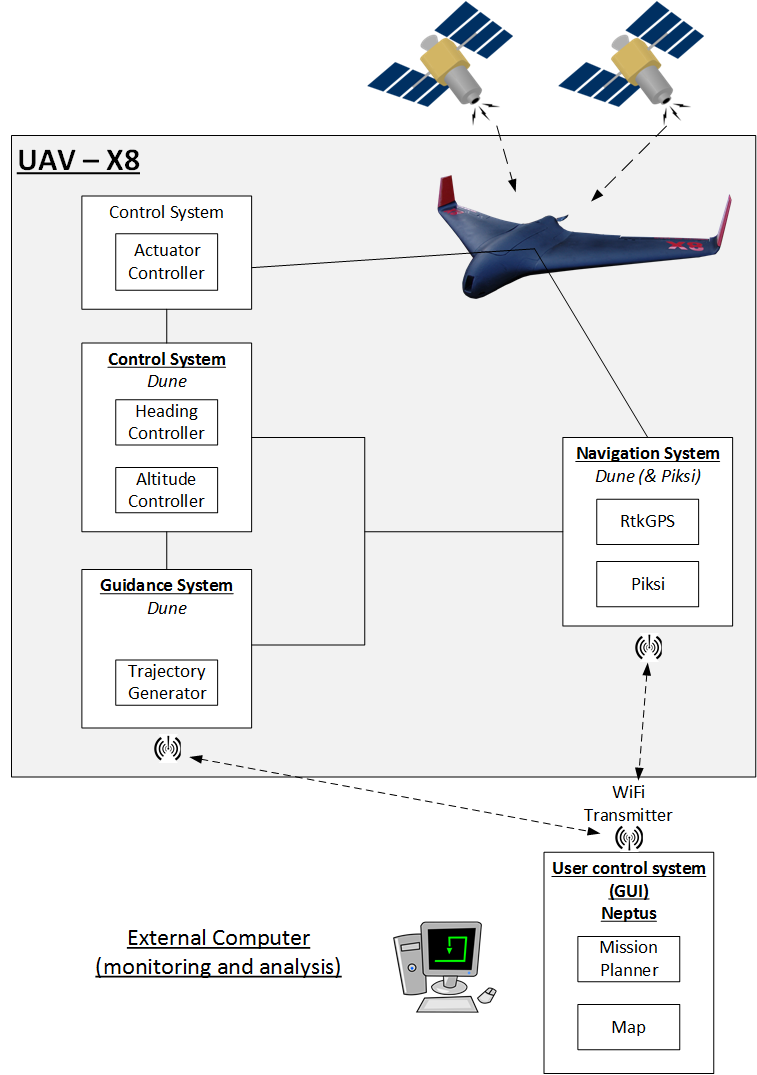
\includegraphics[width=1\textwidth]{figs/System.png}
		\caption{Overview of the automatic net landing system}
		\label{figure:SystemOverview}
\end{figure}

The path planer and the guidance system used as basis for this work were developed as previous master thesis work \citep{Froelich}. A key component in the guidance system is the position estimation system, which was developed in the NTNU MSc thesis \citep{Spockeli}. However, this system has been concluded to be in-sufficient with respect to provide means required for automatic landing.

The control and guidance system has currently only been tested in \gls{sil} simulations with Ardupilot, which shows promising result likely to be sufficient for automatic landing applications. However this module has not yet been implemented to support the use of \gls{rtk-gps} as required for performing automatic landing.

This project work will continue the research done by Spockeli \citep{Spockeli}, and use a new \gls{gnss} receiver, namely the Ublox LEA M8T, that will be used together with the open source program, \gls{rtklib}. The \gls{rtklib} system is compared to the Piksi system from Swift Navigation. The real time position estimate from both systems are compared to a post-processed solution. The goal is to establish a system with accurate local position estimate, such that in the future a \gls{uav} net landing can be performed automatic. The navigation system must be accurate enough to correctly estimate if the \gls{uav} is following the generated landing path or if the deviation from the path is large enough such that an evasion manoeuvre is required. The position evasion criteria used in \citep{Froelich} is $\pm1m$ cross-track error and $\pm1m$ altitude error.
The automatic net landing system will use \gls{rtk-gps} for relative position estimation. The main goal for this work is to describe the gaps of the available position system sufficient to scope further work required for closure of such gaps ultimately providing means for position estimating sufficient for completion of automatic landing.

This work will be done at the UAV-Lab, which is a research lab at NTNU. The UAV-Lab is a test facility for software and hardware, which include inertial navigations system,global satellite navigation systems and unmanned aerial systems.

% This will include:
%\begin{table}[!h]
%\begin{center}
%    \begin{tabular}{ l}
%     Testing of the performance of Ublox LEA M8T  \\ 
%     Compare the performance of \gls{rtklib} and Piksi \\
%     Compare the real time estimate with the post processed estimate 
%    \end{tabular}
%\end{center}
%\label{Tb:Evasion}
%\end{table}
%The scope of this work is to test the performance of ublox-LEA M8T \gls{gnss} receiver in a real time differential \gls{dgps} configuration. The \gls{rtk-gps} solution will be calculated with the open source program \gls{rtklib}, which will communicate with a task in DUNE. The solution from \gls{rtklib} will be compared against the solution from Piksi, and a post processed solution from \gls{rtklib}. The result from the experiment will be used in the discussion on how to perform an automatic net landing.

%For validation of the position accuracy needed the evasion criteria given in \ref{Tb:Evasion} \citep{Froelich} will be used.
%\begin{table}[!h]
%\begin{center}
%    \begin{tabular}{ | l | l |}
%    \hline
%    \textbf{Criteria} & \textbf{Value} \\ \hline
%     Cross-track error & $\pm1$ meter  \\ \hline
%     Altitude error & $\pm1$ meter \\ \hline
%    \end{tabular}
%\end{center}
%\caption{Evasion criteria }
%\label{Tb:Evasion}
%\end{table}

\section{Layout}
This project work contain five chapters and one appendix. The chapter are indexed 1-5, and the appendix are indexed A. A short description of the chapters and appendix are given below.
\begin{itemize}
\item Chapter 2 \gls{uav} navigation system: Contains a general description of the \acrfull{gps}, in addition to how \gls{gps} is used in the navigation system.
\item Chapter 3 System components and implementation: Describes the software and hardware components used in the navigation system, in addition to the implementation into the navigation system.
\item Chapter 4 Experimental testing: Present the experimental results.
\item Chapter 5 Closing discussion and conclusion: Summarize the conclusions draw from the result and provide recommendation for further work.
\item Appendix A RTKLIB configuration: Present the configuration file for \gls{rtklib}

\end{itemize}
\cleardoublepage